\part{Week 5}
\chapter{Entropy and information}
We know that \textit{entropy} measures uncertainity of state of a physical system. We'll look into it's definitions and properties deeply both in classical and quantum information theory.

\section{Shannon entropy}
It's the key concept of classical information theory. It can be viewed in two complementary views, first, suppose we have a random variable $X$, how much information we \textit{gain} on average if we know the value of $X$. Second, it's the measure of \textit{uncertainity} before we know the value of $X$.

Information content of a random variable doesn't depend on labels. For example, a random variaible giving `heads' and `tails' with probability $1/4$ and $3/4$ contains same information as a random variable giving `$0$' and `$1$' with probability $1/4$ and $3/4$ respectively. Thus, entropy also doesn't depend on labels. \textit{Shannon entropy} associated with a probability distribution $p_1,\dots,p_n$ is given by
\begin{equation}
    H(X) \equiv H(p_1,\dots,p_n) \equiv -\sum_x p_x\log p_x
\end{equation}
Note that by $\log$ we mean base $2$, by $\ln$ we mean base $e$. Since a never occuring event with probability $p_i=0$ should never affect entropy, thus we agree that $0\log 0=0$ even though we mean $\lim_{x\rightarrow0} x\log x = 0$. There's a nice reason why entropy is defined this way. We have to \textit{quantify the resources needed to store information}. Let's suppose a source producing symbols $X_1,X_2,\dots$ of independent \textit{identically} distributed random variables, minimal amount of resources required to store the information produced by source such that it can be reconstructed turns out to be just entropy i.e $H(X)\equiv H(X_1) \equiv H(X_2) = \dots$, this result is known as \textit{Shannon's noiseless coding theorem}.

I suggest looking at an example to understand this. Suppose our source produces $1$, $2$, $3$, $4$ which are symbols but with probability $1/2$, $1/4$, $1/8$ and $1/8$ respectively. We don't need two bits to store output of each use of source. We can compress this usage, by representing $1$ as $0$, $2$ as $10$, $3$ as $110$ and $4$ as $111$, with this we can reconstruct the message, for eg. $11010111$ as $324$ too. We need on an average $\frac{1}{2}\cdot 1 + \frac{1}{4}\cdot 2 + \frac{1}{8}\cdot 3 + \frac{1}{8}\cdot 3 = 7/4$ bits only! It also turns out that this is just the entropy of the source $H(X) = -1/2\log(1/2) - 1/4\log(1/4) - 1/8\log(1/8) - 1/8\log(1/8) = 7/4$. It's also true that average information gained by an event out of a probability distribution $p_1,\dots,p_n$ is $k\sum_ip_i\log p_i$ for some constant $k$.

\section{Basic properties of entropy}
\subsection{The binary entropy}
The entropy of a two-outcome random variable is so special that we name it as \textit{binary entropy}
\begin{equation}
    H_{\text{bin}}(X) \equiv -p\log p - (1-p)\log (1-p)
\end{equation}
where $p$ and $1-p$ are probabilities of outcome. It's graph is shown in figure  \ref{fig:binary-entropy} 
\begin{figure}
    \centering
    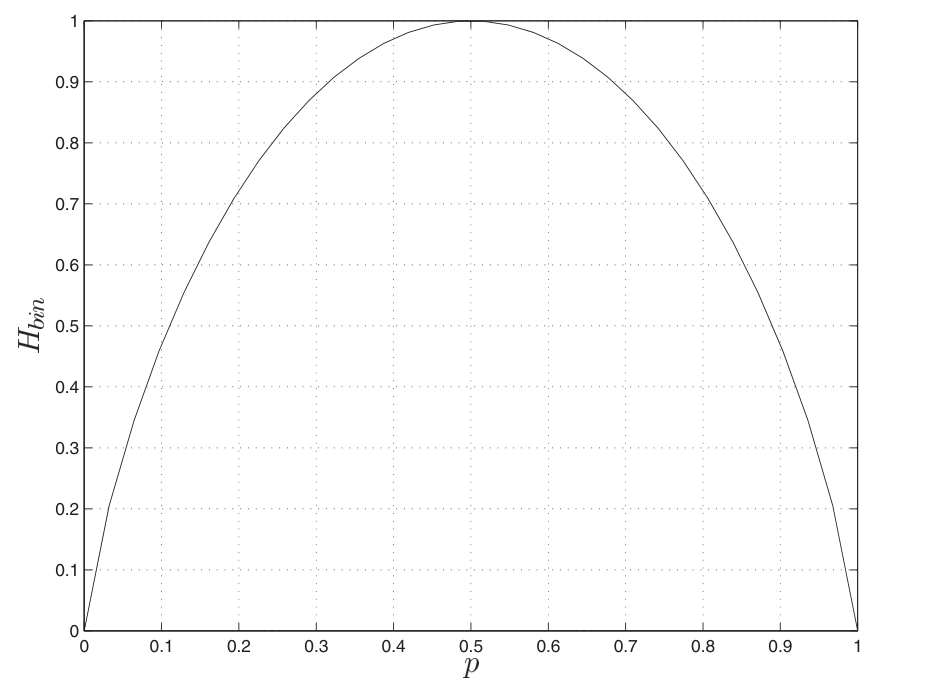
\includegraphics[width=0.65\textwidth]{images/binary_entropy.png}
    \caption{Binary entropy function $H(p)$}
    \label{fig:binary-entropy}
\end{figure}

A really good intuition comes when we consider this example of Alice having two biased coins one from US and another from Australia. Suppose the US coin gives head with probability $p_U$ and the Australian coin with probability $p_A$ and Alice flips one of those coins with probability $q$ for US coin and $1-q$ for Australian coin and she tells final `head' or `tail' to Bob. The information Bob gets is atleast the average information he gets from flipping one coin. Hence
\begin{equation}
    H(qp_U + (1-p)p_A) \geq qH(p_U) + (1-q)H(p_A)
\end{equation}
It's greater because Bob gets \textit{more} information about the country sometimes. For eg. if $p_U=0.1$ and $p_A=0.9$ and Alice says head, Bob would understand that it's more probable to be an aussie coin. This leads us into a very important property of entropy, \textit{concavity}. Which can be seen in binary case in the figure \ref{fig:binary-entropy}.

\subsection{The relative entropy}
The \textit{relative entropy} is useful entropy-like measure describing closeness of two probability distributions $p(x)$ and $q(x)$ over the same index set $x$, defined by
\begin{equation}
    H(p(x) \parallel q(x)) \equiv \sum_x p(x)\log \frac{p(x)}{q(x)} \equiv -H(X)-\sum_x p(x)\log q(x)
\end{equation}
The following theorem motivates us to understand it as a distance measure
\begin{theorem}[\textbf{Non-negativity of relative entropy}]
    The relative entropy is non-negative, $H(p(x) \parallel q(x)) \geq 0$ with equality if and only if $p(x)=q(x)$ for all $x$.
    \label{thm:non-negativity-of-rel-entropy}
\end{theorem}
The proof is simple using the definition of relative entropy and $\log x \ln{2} \leq x-1$ with equality only when $x=1$. Relative entropy itself is not very useful but used to study entropy, for example let $q(x)$ be uniform probability distribution over index set $X$ of size $d$ then for a probability distribution $p(x)$ over $X$, we have
\begin{equation}
    H(p(x)\parallel q(x)) = H(p(x)\parallel 1/d) = -H(X) - \sum_x p(x) \log (1/d) = \log d - H(X)
\end{equation}
and hence by theorem \ref{thm:non-negativity-of-rel-entropy} we have $\log d - H(X) \geq 0$ thus $H(X) \leq \log d$, a nice property hence a theorem!
\begin{theorem}
    Suppose $X$ is a random variable with $d$ outcomes. Then $H(X) \leq \log d$, with equality if and only if $X$ is uniformly distributed over those $d$ outcomes.
\end{theorem}

\subsection{Conditional entropy and mutual information}
For two random variables $X$, $Y$ we'll try to understand how information of $X$ is related to that of $Y$. First we define \textit{joint entropy} of $X$ and $Y$ as
\begin{equation}
    H(X, Y) \equiv -\sum_{x, y} p(x, y)\log p(x, y)
\end{equation}
The \textit{entropy of $X$ conditional on knowing $Y$} is similar to that in probability, it's the uncertainity that we have in the value of $X$ given that we know the value of $Y$. It's defined by
\begin{equation}
    H(X | Y) \equiv H(X,Y) - H(Y)
\end{equation}

A second quantity \textit{mutual information content of $X$ and $Y$} measures how much information $X$ and $Y$ have in common. It's very similar to intersection, given we take $H(X,Y)$ as information content of both $X$ and $Y$ which is counted twice. Thus, mutual information content is
\begin{equation}
    H(X:Y) = H(X) + H(Y) - H(X, Y)
\end{equation}
The relation $H(X:Y) = H(X) - H(X|Y)$ also comes in handy. Let's see some more simple relationships between different entropies.

\begin{ntheorem}[\textbf{Basic properties of Shannon entropy}]
    \begin{enumerate}
        \item $H(X, Y) = H(Y, X), H(X:Y) = H(Y:X)$
        \item $H(Y|X) \geq 0$ and thus $H(X:Y)\leq H(Y)$ with equality if and only if $Y$ is a function of $X$, $Y=f(X)$.
        \item $H(X) \leq H(X,Y)$ with equality if and only if $Y$ is a function of $X$.
        \item \textbf{Subadditivity:} $H(X, Y) \leq H(X) + H(Y)$ with equality if and only if $X$ and $Y$ are independent variables.
        \item $H(Y|X) \leq H(Y)$ and thus $H(X:Y) \geq 0$ with equality in each if and only if $X$ and $Y$ are independent distributions.
        \item \textbf{Strong subadditivity:} $H(X,Y,Z) + H(Y) \leq H(X,Y) + H(Y, Z)$, with equality if and only if $Z\rightarrow Y\rightarrow X$ forms a markov chain.
        \item \textbf{Conditioning reduces entropy:} $H(X|Y,Z) \leq H(X|Y)$.
    \end{enumerate}
\end{ntheorem}
All this can be easily understood by a Venn diagram for entropy.
\begin{figure}[H]
    \centering
    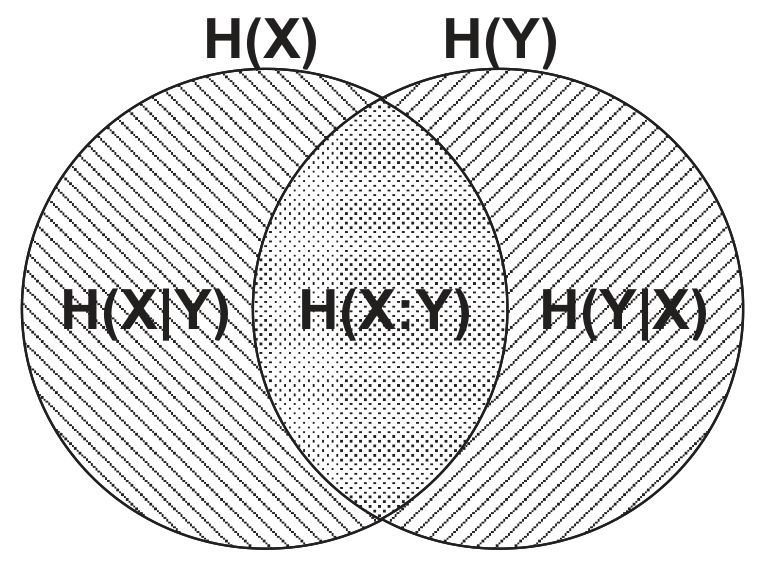
\includegraphics[width=0.45\textwidth]{images/venn_entropy.png}
    \caption{Relationships between different entropies}
    \label{fig:venn-entropy}
\end{figure}
Let's finally consider a simple and useful chaining rule for conditional entropies.
\begin{theorem}
    Let $X_1,\dots,X_n$ and $Y$ be any set of random variables. Then
    \begin{equation}
        H(X_1,\dots,X_n|Y) = \sum_{i=1}^n H(X_i|Y,X_1,\dots,X_{i-1})
    \end{equation}
\end{theorem}
\begin{proof}
    Use induction with base case $n=2$.
\end{proof}

\subsection{The data processing inequality}
